\documentclass[oneside,a4paper,11pt]{book}      
% \documentclass[twoside,a4paper,11pt]{book}


\usepackage{fancyhdr}
\setlength{\headheight}{15pt}
\usepackage[pdftex,
pdfauthor={Name, Vorname},
pdftitle={Überschrift},
pdfsubject={Projektarbeit},
pdfkeywords={Unterschrift}
]{hyperref}
\usepackage[ngerman]{babel}
\usepackage[T1]{fontenc}
\usepackage[utf8]{inputenc}
\usepackage[dvips]{graphicx}
\usepackage{calc}
\usepackage{makeidx}
\usepackage{xcolor}
\usepackage[hang,small,scriptsize,bf]{caption}
\usepackage{amssymb}
\usepackage{subcaption}
\usepackage{hyperref}
\usepackage{multirow}
\usepackage{circuitikz}
\usepackage{seqsplit}
\usepackage[normalem]{ulem}
\usepackage[
  style=numeric,
  sorting=none,
  backend=biber
  ]{biblatex}
  \addbibresource{Literaturverzeichnis.bib}

\usepackage{csquotes}

\usepackage{animate}


\usepackage{hsel-thesis2020}
%
%% ----------------------------------------------------
% enable and define uniform style for code listings
%% ----------------------------------------------------
\usepackage{listings}
\usepackage{caption}

% define colors for syntax highlighting
\definecolor{dkgreen}{rgb}{0,.6,0}
\definecolor{dkblue}{rgb}{0,0,.6}
\definecolor{dkyellow}{cmyk}{0,0,.8,.3}
\definecolor{dkred}{rgb}{0.6,0,0}

\lstset{
	language=C++,	% override by '\begin{lstlisting}[language=...' 
	frame=single, 	% top,frame=bottom,
	numbers=left,
	numberstyle=\tiny\color{gray!90!black},
	basicstyle=\ttfamily\footnotesize,
	tabsize=2,
	showstringspaces=false,
	captionpos=t,
  % postbreak=\mbox{\textcolor{red}
  % morekeywords={self},              % Add keywords here
  otherkeywords={self},              % Add keywords here
  emph={Robot,__init__,__del__},          % Custom highlighting
  emphstyle=\color{dkred},    % Custom highlighting style
	rulecolor=\color{lightgray!40},
	keywordstyle=\color{dkblue},
	stringstyle=\color{red},
	commentstyle=\color{dkgreen},
  breaklines=true,
}

\DeclareCaptionFormat{listing}{	\par\vskip1pt#1#2#3}
\captionsetup[lstlisting]
{
	format=listing,
	singlelinecheck=false, 
	margin=1em, 	
	labelsep=colon,
	justification=centering
	%font={sf},
	%labelfont=bf
}


% \lstdefinestyle{mymypython}{
%   %\lstset{
%   %keepspaces=true,
%   language=python,
%   showtabs=true,
%   tab=,
%   tabsize=2,
%   basicstyle=\ttfamily\footnotesize,%\setstretch{.5},
%   stringstyle=\color{stringcolour},
%   showstringspaces=false,
%   alsoletter={1234567890},
%   otherkeywords={\%, \}, \{, \&, \|},
%   keywordstyle=\color{keywordcolour}\bfseries,
%   emph={and,break,class,continue,def,yield,del,elif ,else,%
%   except,exec,finally,for,from,global,if,import,in,%
%   lambda,not,or,pass,print,raise,return,try,while,assert,with},
%   emphstyle=\color{blue}\bfseries,
%   emph={[2]True, False, None},
%   emphstyle=[2]\color{keywordcolour},
%   emph={[3]object,type,isinstance,copy,deepcopy,zip,enumerate,reversed,list,set,len,dict,tuple,xrange,append,execfile,real,imag,reduce,str,repr},
%   emphstyle=[3]\color{commandcolour},
%   emph={Exception,NameError,IndexError,SyntaxError,TypeError,ValueError,OverflowError,ZeroDivisionError},
%   emphstyle=\color{exceptioncolour}\bfseries,
%   %upquote=true,
%   morecomment=[s]{"""}{"""},
%   commentstyle=\color{commentcolour}\slshape,
%   %emph={[4]1, 2, 3, 4, 5, 6, 7, 8, 9, 0},
%   emph={[4]ode, fsolve, sqrt, exp, sin, cos,arctan, arctan2, arccos, pi,  array, norm, solve, dot, arange, isscalar, max, sum, flatten, shape, reshape, find, any, all, abs, plot, linspace, legend, quad, polyval,polyfit, hstack, concatenate,vstack,column_stack,empty,zeros,ones,rand,vander,grid,pcolor,eig,eigs,eigvals,svd,qr,tan,det,logspace,roll,min,mean,cumsum,cumprod,diff,vectorize,lstsq,cla,eye,xlabel,ylabel,squeeze},
%   emphstyle=[4]\color{numpycolour},
%   emph={[5]__init__,__add__,__mul__,__div__,__sub__,__call__,__getitem__,__setitem__,__eq__,__ne__,__nonzero__,__rmul__,__radd__,__repr__,__str__,__get__,__truediv__,__pow__,__name__,__future__,__all__},
%   emphstyle=[5]\color{specmethodcolour},
%   emph={[6]assert,yield},
%   emphstyle=[6]\color{keywordcolour}\bfseries,
%   emph={[7]range},
%   emphstyle={[7]\color{keywordcolour}\bfseries},
%   % emph={[7]self},
%   % emphstyle=[7]\bfseries,
%   literate=*%
%   {:}{{\literatecolour:}}{1}%
%   {=}{{\literatecolour=}}{1}%
%   {-}{{\literatecolour-}}{1}%
%   {+}{{\literatecolour+}}{1}%
%   {*}{{\literatecolour*}}{1}%
%   {**}{{\literatecolour{**}}}2%
%   {/}{{\literatecolour/}}{1}%
%   {//}{{\literatecolour{//}}}2%
%   {!}{{\literatecolour!}}{1}%
%   %{(}{{\literatecolour(}}{1}%
%   %{)}{{\literatecolour)}}{1}%
%   {[}{{\literatecolour[}}{1}%
%   {]}{{\literatecolour]}}{1}%
%   {<}{{\literatecolour<}}{1}%
%   {>}{{\literatecolour>}}{1}%
%   {>>>}{\pythonprompt}{3}%
%   ,%
%   %aboveskip=.5ex,
%   frame=trbl,
%   %frameround=tttt,
%   %framesep=.3ex,
%   rulecolor=\color{black!40},
%   %framexleftmargin=\framemargin,
%   %framextopmargin=.1ex,
%   %framexbottommargin=.1ex,
%   %framexrightmargin=\framemargin,
%   %framexleftmargin=1mm, framextopmargin=1mm, frame=shadowbox, rulesepcolor=\color{blue},#1
%   %frame=tb,
%   backgroundcolor=\color{white},
%   breakindent=.5\textwidth,frame=single,breaklines=true%
%   %}
% }


% Kombination von \textit und \textbf
\newcommand{\textbfit}[1]{\textbf{\textit{#1}}}

\begin{document}

\AddToShipoutPicture{\BackgroundWave}
\pagenumbering{Roman}

\begin{titlepage}

	\vspace{-0.5cm}
	\hspace{-3.0cm}
	% \hspace{-2.0cm}
	\begin{tabular}{p{8.0cm} p{8.0cm}}
		
\includegraphics[width = 6.0cm]{img/GUI/hsel-allgemein} &
		\parbox[b]{8.0cm}{
		{\large 	Fachbereich Technik }                            \\
		{\large 	Abteilung Elektrotechnik und Informatik }
		}                                                         \\
		\\
		\hline
	\end{tabular}
	%
	\begin{center}

		\vspace{2.5cm}
		\LARGE{\textsc{
				Hyperloop\\
				48 V
			}}\\

		\vspace{2.5cm}
		\LARGE{\textsc{
				{Projektarbeit}
			}}\\
		\large
		Studiengang Elektrotechnik

		\vspace{2cm}%
		\large
		Vorgelegt von\\ Oliver, Schmidt\\ Studiengang Elektrotechnik\\ Matr. Nr. 7023462

		\vspace{1cm}
		Emden, \today

		\vspace{3.5cm}%
		Betreut von\\ Prof. Dr.-Ing. Kane

	\end{center}
	\normalsize
\end{titlepage}

\linespread{1.2}
\noitemsep
\include{source/0_1_RechtlicheErklärung}
\tableofcontents
\listoffigures
\label{sec:Abbildungsverzeichnis}
\addcontentsline{toc}{section}{Abbildungsverzeichnis}



\listoftables
\label{sec:Tabellenverzeichnis}
\addcontentsline{toc}{section}{Tabellenverzeichnis}

\listofscheme
\label{sec:Diagrammverzeichnis}
\addcontentsline{toc}{section}{Diagrammverzeichnis}

\listofoszillo
\label{sec:Oszillogrammverzeichnis}
\addcontentsline{toc}{section}{Oszillogrammverzeichnis}



%\lstlistoflistings
%\label{sec:Codeverzeichnis}
%\addcontentsline{toc}{section}{Code Listings}

\newpage


\cleardoublepage
\pagenumbering{arabic}
\ClearShipoutPicture


\chapter{Einleitung}
\label{chapter:Einleitung}

\section{Motivation}
\label{section:Motivation}

Der Hyperloop ist ein innovatives Transportkonzept, das eine ökonomische, klimafreundliche und schnellere Alternative zu herkömmlichen Verkehrsmitteln wie Lastkraftwagen, Zügen und Flugzeugen bietet.
Derzeit stehen herkömmlichen Transportmitteln zwei wesentliche Hindernisse im Weg, um Personen und Güter schnell und emissionsarm zu befördern: Zum einen der hohe Luftwiderstand, der bei hohen Geschwindigkeiten den Energieverbrauch stark erhöht, und zum anderen der Rollwiderstand der Räder, der ebenfalls zu einem höheren Energiebedarf führt.
\begin{figure}[!ht]
	\begin{center}
		\includegraphics[width=1\textwidth]{img/1_strecke/strecke_1.png}
		\caption{Hyperloop der Hochschule Emden-Leer}
		\label{img_1_1:strecke}
	\end{center}
\end{figure}
\pagebreak[1]


Der Hyperloop löst diese Probleme, indem er Güter und Personen in einem Fahrzeug, das sich in einer Vakuumröhre bewegt, wie in Abbildung \ref{img_1_1:strecke} dargestellt ist, zudem wird das Fahrzeug, wie bei einer Magnetschwebebahntechnik angehoben, somit lassen sich Roll- und Luftwiderstand fast vollkommen aufheben.

Angesichts der globalen Bemühungen zur Reduzierung der CO2-Emissionen und zur Bekämpfung des Klimawandels könnte Hyperloop eine umweltfreundlichere Alternative zu Autos und Flugzeugen bieten.





\subsection{Institute of Hyperloop Technology}
\label{section:IHT}

\textbf{\textcolor{red}{Zitieren!!!!!!}}\\ \ \\
Die Hochschule Emden/Leer hat im Jahr 2021 das Institut für Hyperloop-Technologie (IHT) gegründet, um aktiv an der Forschung zu dieser zukunftsweisenden Technologie teilzunehmen.

Im Rahmen dieser Forschung wurde an der Hochschule Emden eine Teststrecke mit einer Länge von 26 Metern errichtet (siehe Abbildung \ref{img_1_1:strecke}). Auf dieser Strecke soll das Fahrzeug (POD) unter realistischen Bedingungen getestet und weiterentwickelt werden.
Die Teststrecke besteht aus einem Schinensystem und einem Linarmotor. Der Linarmotor wird für die Magnetschwebebahntechnik verwendet.


Darüber hinaus engagiert sich das IHT in verschiedenen Projekten, darunter das \frqq European Hyperloop Technology Center – EuHyTeC\flqq, das europäische Hyperloop-Initiativen vernetzt und gemeinsam die nächste Generation des Transports entwickelt.
\newpage




\section{Aufgabenstellung}
\label{section:Aufgabenstellung}

\myboxy{
	\begin{itemize}
		\item Ablauforientiert erklären. Also erst die Bestellung, dann der Schaltplan und dann die Simulation mit Simulink.
		\item Aufgabenstellung in der Vergangenheit formulieren.
		\item Den Leser in der Doku struktur Einführen. Am enden in 1.x
	\end{itemize}
}{To-do}{\textwidth}


Die Motivation für dieses Projekt liegt in der Entwicklung eines Hyperloop-Fahrzeugs, das mit einer Batterie und einem Motor betrieben wird. Für die Steuerung des Fahrzeuges wurde ein echtzeitfähiges Steuerungsystem der Firma Speedgoat vorgeben, welches in Abschnitt \ref{section:speedgoat} vertieft wird.\\ \ \\

Im Rahmen des Projekts wird ein Fahrzeug (Pod) für den Hyperloop mit einer Bordspannung von 48 V konzipiert. Ziel ist es, die Machbarkeit dieser Spannung zu überprüfen und umzusetzen. Dazu gehören die Planung und Simulierung, die Integration der erforderlichen Sensorik sowie die Beschaffung der notwendigen Bauteile. Die Logik- und Signalverarbeitung wird mithilfe von Simulink auf dem echtzeitfähigen Speedgoat-System durchgeführt.
Die Steuerung erfolgt über Simulink, ein Modul von MATLAB, und umfasst die Erfassung von Position und Beschleunigung des Fahrzeuges. Der Motor wird über ein zusätzliches Steuergerät angesteuert. Die Steuerung soll als Automatensteuerung umgesetzt werden.
Die Verdrahtung des Pods wird entsprechend der Bordspannung von 48 V ausgelegt. Hierfür wird mit der Software QElectroTech ein Schaltplan erstellt.
Alle erforderlichen Bauteile für die Umsetzung der Bordspannung, die Verdrahtung und die Sensorik müssen beschafft werden.
Textergebnisse und in Betriebnahme entfallen.


\section{Aufbau der Projektdokumentation}
\label{section:Aufbau}

\chapter{Verwendet Technik}

\section{Konzept}
Der Pod wird von einem BLDC-Motor angetrieben, wobei die elektrische Energie in einem Lithium-Ionen-Akku gespeichert wird. Der Motor wird durch einen Sinuswellen-Generator gesteuert. Mit dem Speedgoat-System werden die Eingangssignale des Sinuswellen-Generators sowie andere Aktoren gesteuert.

\section{Antrieb}
\label{Golden_Motor}
Golden Motor ist ein Anbieter von Elektromotoren und elektrischen Antriebssystemen. Das Unternehmen bietet eine breite Palette von Produkten an, darunter:
Motoren und Komplettsysteme für Elektrofahrräder, Industrielle BLDC-Motoren, Elektrische Antriebe für Boote.


\subsection{BLDC Motor}
\label{BLDC_Motor}


Ein BLDC-Motor (Brushless DC Motor) unterscheidet sich grundlegend von einem herkömmlichen Gleichstrommotor. Während bei einem traditionellen DC-Motor die Polumschaltung (Kommutierung) mechanisch über Kohlebürsten erfolgt, übernimmt beim BLDC-Motor eine elektronische Steuerung diese Aufgabe. Dadurch entfällt die Notwendigkeit von Kohlebürsten, was den Motor effizienter und langlebiger macht\cite{mathworks:bldc_motor}.

\begin{figure}[ht]
	\begin{center}
		\includegraphics[width=\textwidth]{img/2_antrieb/motor_1.png}
		\caption{Golden Motors – 10 KW BLDC Motor Liquid Cooled}
		\label{img_2_2:antrieb_motor:1}
	\end{center}
\end{figure}
\pagebreak[4]


Die Anschlüsse des BLDC-Motors sind in Abbildung \ref{img_2_2:circ_bldc:1} dargestellt. Der Motor verfügt über zwei Ausgänge, die jeweils mit drei Hall-Sensoren ausgestattet sind, sowie über einen Temperatursensor. Zusätzlich werden über das Kabel ein GND und eine +5V-Versorgung benötigt. Die Spulen des Motors werden über drei Phasen angeschlossen: U, V und W.

\begin{figure}[ht]
	\begin{center}
		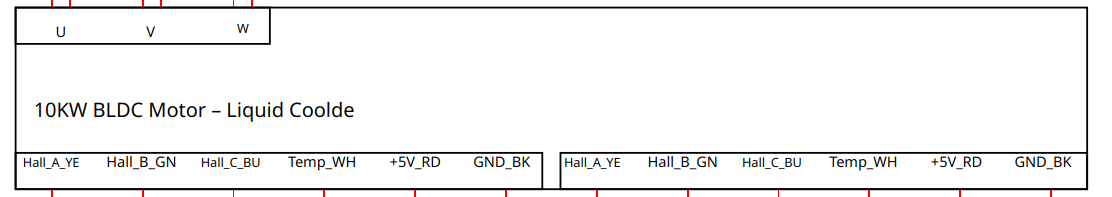
\includegraphics[width=\textwidth]{img/2_imp/2_circ_bldc_motor.png}
		\caption{Zeichnung: BLDC Motor}
		\label{img_2_2:circ_bldc:1}
	\end{center}
\end{figure}
\newpage



\subsection{Vector Controller}
Der Vector Controller verwendet die Motorsteuerungstechnologie feldorientierte Regelung (Field-Oriented Control - FOC), dass bedeutet das der Controller mittels den Hallsensoren, ein Rückgekoppelten Regelkreis bildet und somit die Lage des Polrades ermittelt.

\cite{schroeder:elektische_antriebe}

Sie bietet eine effiziente Steuerung von BLDC-Motoren in Anwendungen mit variabler Drehzahl und schnell wechselnden Lasten und verbessert die Energieeffizienz von Asynchronmotoren, vor allem bei niedrigen Drehzahlen.


\begin{figure}[ht]
	\begin{center}
		\includegraphics[width=\textwidth]{img/2_antrieb/sine_1.png}
		\caption{Golden Motors – VECTOR 500 Motor Controller}
		\label{img_2_2:antrieb_sine:1}
	\end{center}
\end{figure}


%Dafür muss der Abstand ermittelt werden, dies wird mit einem Abstandslaser gemacht.

%Die Steuerung wird als Automaten umgesetzt. Dabei werden unterschiedliche Zustände durchlaufen, wie Idel, Drive, Distance und Stop.
\section{Steuerung – Speedgoat}

Speedgoat ist ein Unternehmen, das sich auf die Entwicklung und den Vertrieb von echtzeitfähigen modellbasierten Design-Workflows spezialisiert hat, die vor allem in der Steuerungs- und Regelungstechnik eingesetzt werden.
Speedgoat arbeitet eng mit MATLAB und Simulink zusammen und bietet maßgeschneiderte Hardware-Lösungen, die perfekt auf diese Softwareplattformen abgestimmt sind.

\begin{figure}[ht]
	\begin{center}
		\includegraphics[width=\textwidth]{img/2_steuerung/goat_1.png}
		\caption{Speedgoat}
		\label{img_2_2:steuerung_goat:1}
	\end{center}
\end{figure}


\section{Abstandsmessung}

\begin{figure}[ht]
	\begin{center}
		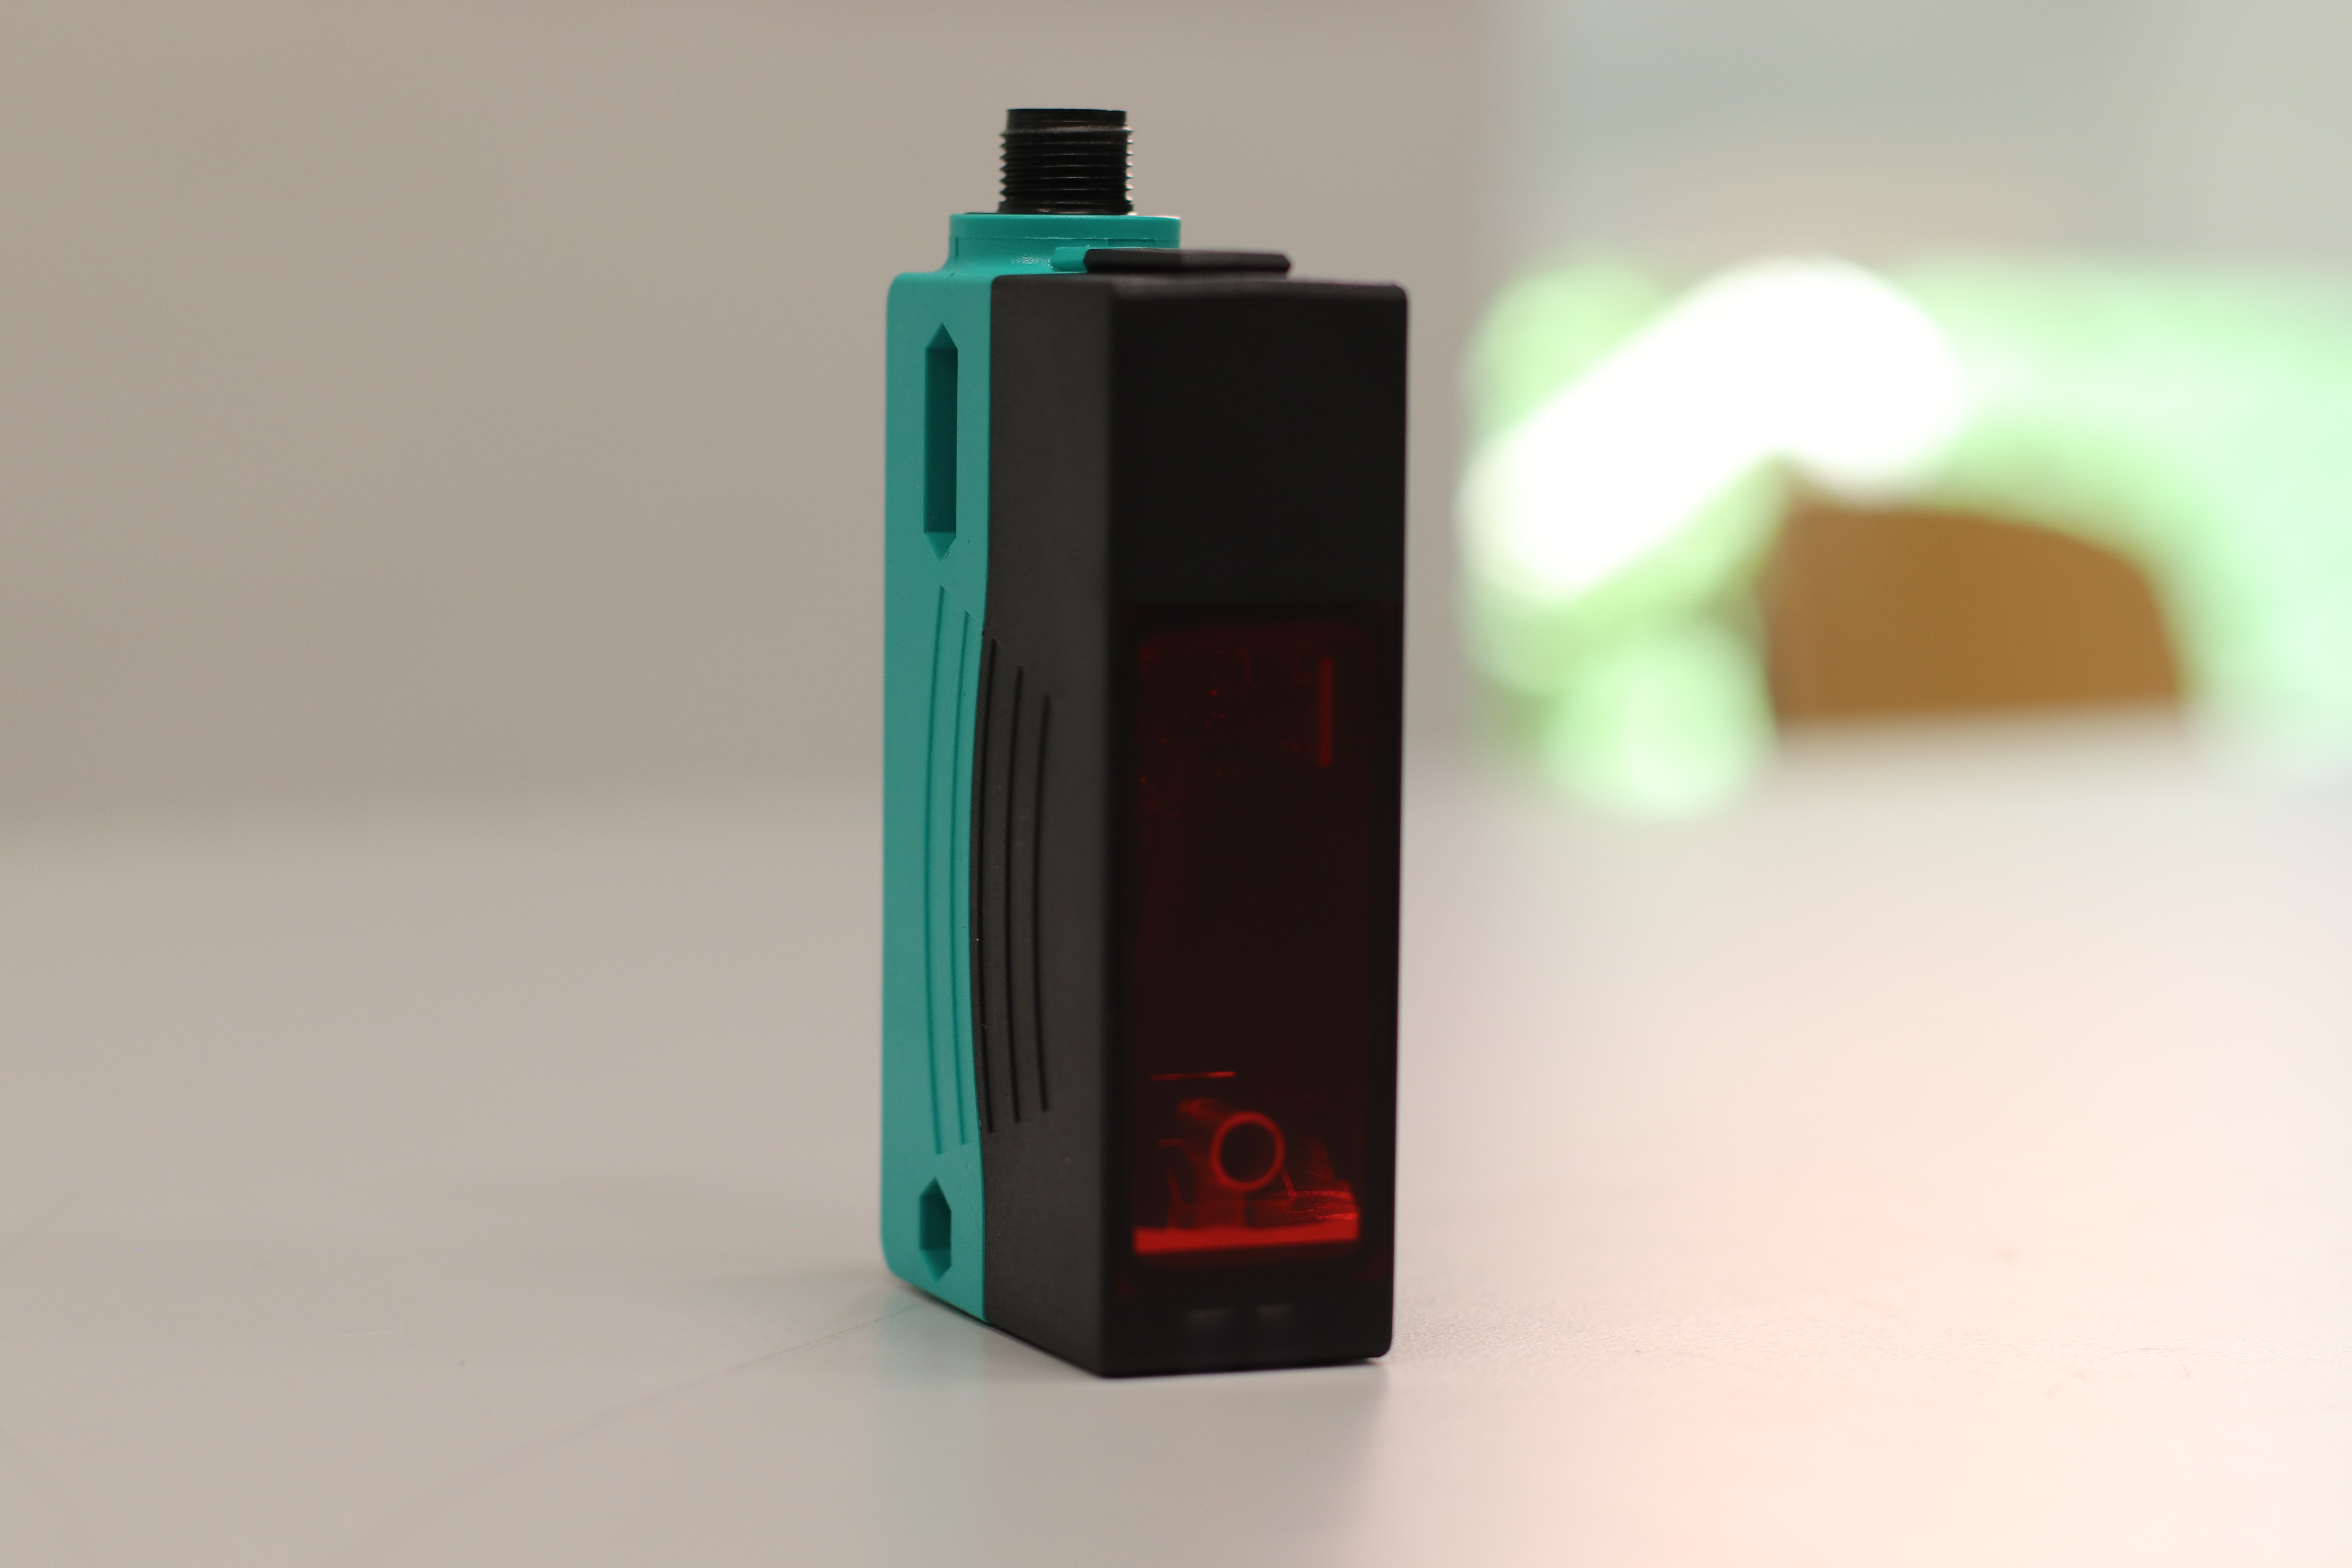
\includegraphics[width=\textwidth]{img/2_sen/dis_1.png}
		\caption{Speedgoat – Baseline Real-Time Target Machine}
		\label{img_2_2:sen_dis:1}
	\end{center}
\end{figure}




\section{Speicher}

\begin{figure}[!ht]
	\begin{center}
		\includegraphics[width=\textwidth]{img/2_speicher/speicher.png}
		\caption{DeepCPower – Lithium Batterie 50Ah | 51,2V | 2560Wh}
		\label{img_2_2:speicher_1:1}
	\end{center}
\end{figure}



\chapter{Implementierung}

\section{Bauteile}

Für das Projekt wurde der die echtzeitfähige steuerung, Batterie,  Motor und dem dazugöhrige Steuerung vorgeben.  Alle weiteren Bauteile mussten bestellt werden. 

\section{Schaltplan}


\subsection{Bauteil erstellung}

Für die erstellung des Schaltpalnes, müssen die Bauteile, die nicht der Norm entsprechen, selber erstellt werden. Alle anschlüsse müssen ermittelt werden und die dazugehörige Funktion ebenso.


\section{Distanzmessung}

Der Sensor von Pepperl+Fuchs wurde ursprünglich für die Distanzmessung angeschafft. Da dieser Sensor jedoch sehr teuer ist und wir nicht das Risiko eines möglichen Schadens im Vakuum eingehen wollten, wurde nach einer kostengünstigen Alternative gesucht.\\
Die Idee bestand darin, ein Entfernungsmessgerät von PARKSIDE zu verwenden und den Sensor aus dem Gerät zu entfernen. Die Messwerte werden anschließend mit einer MCU decodiert.

\subsection{Verbindung}
Der Sensor ist über ein Flachbandkabel mit der Hauptplatine verbunden, wie in Abbildung \ref{img_2_2:sen_dis_parkside:1} zu sehen ist. Auf der Hauptplatine befinden sich vier ungenutzte Lötstellen. Mithilfe eines Oszilloskops haben wir diese Lötstellen analysiert und festgestellt, dass Leitung eins eine Spannung von 3,3 V führt und Leitung vier als GND dient. Die Leitungen zwei und drei übertragen digitale Signale und fungieren als Datenleitungen.\\
Wenn zwei Leitungen für die Datenübertragung vorhanden sind, kann die Kommunikation bei einer zweiadrigen Verbindung entweder synchron oder asynchron erfolgen. Ist die Kommunikation synchron, dient eine der Leitungen als Taktleitung (Clock). Andernfalls, bei einer asynchronen Kommunikation, ist eine Leitung der Sender (TX) und die andere der Empfänger (RX). Dies ermöglicht eine Vollduplex-Übertragung.
Der Sensor komuniziert mit einem Bussystem.




\begin{figure}[ht]
	\begin{center}
		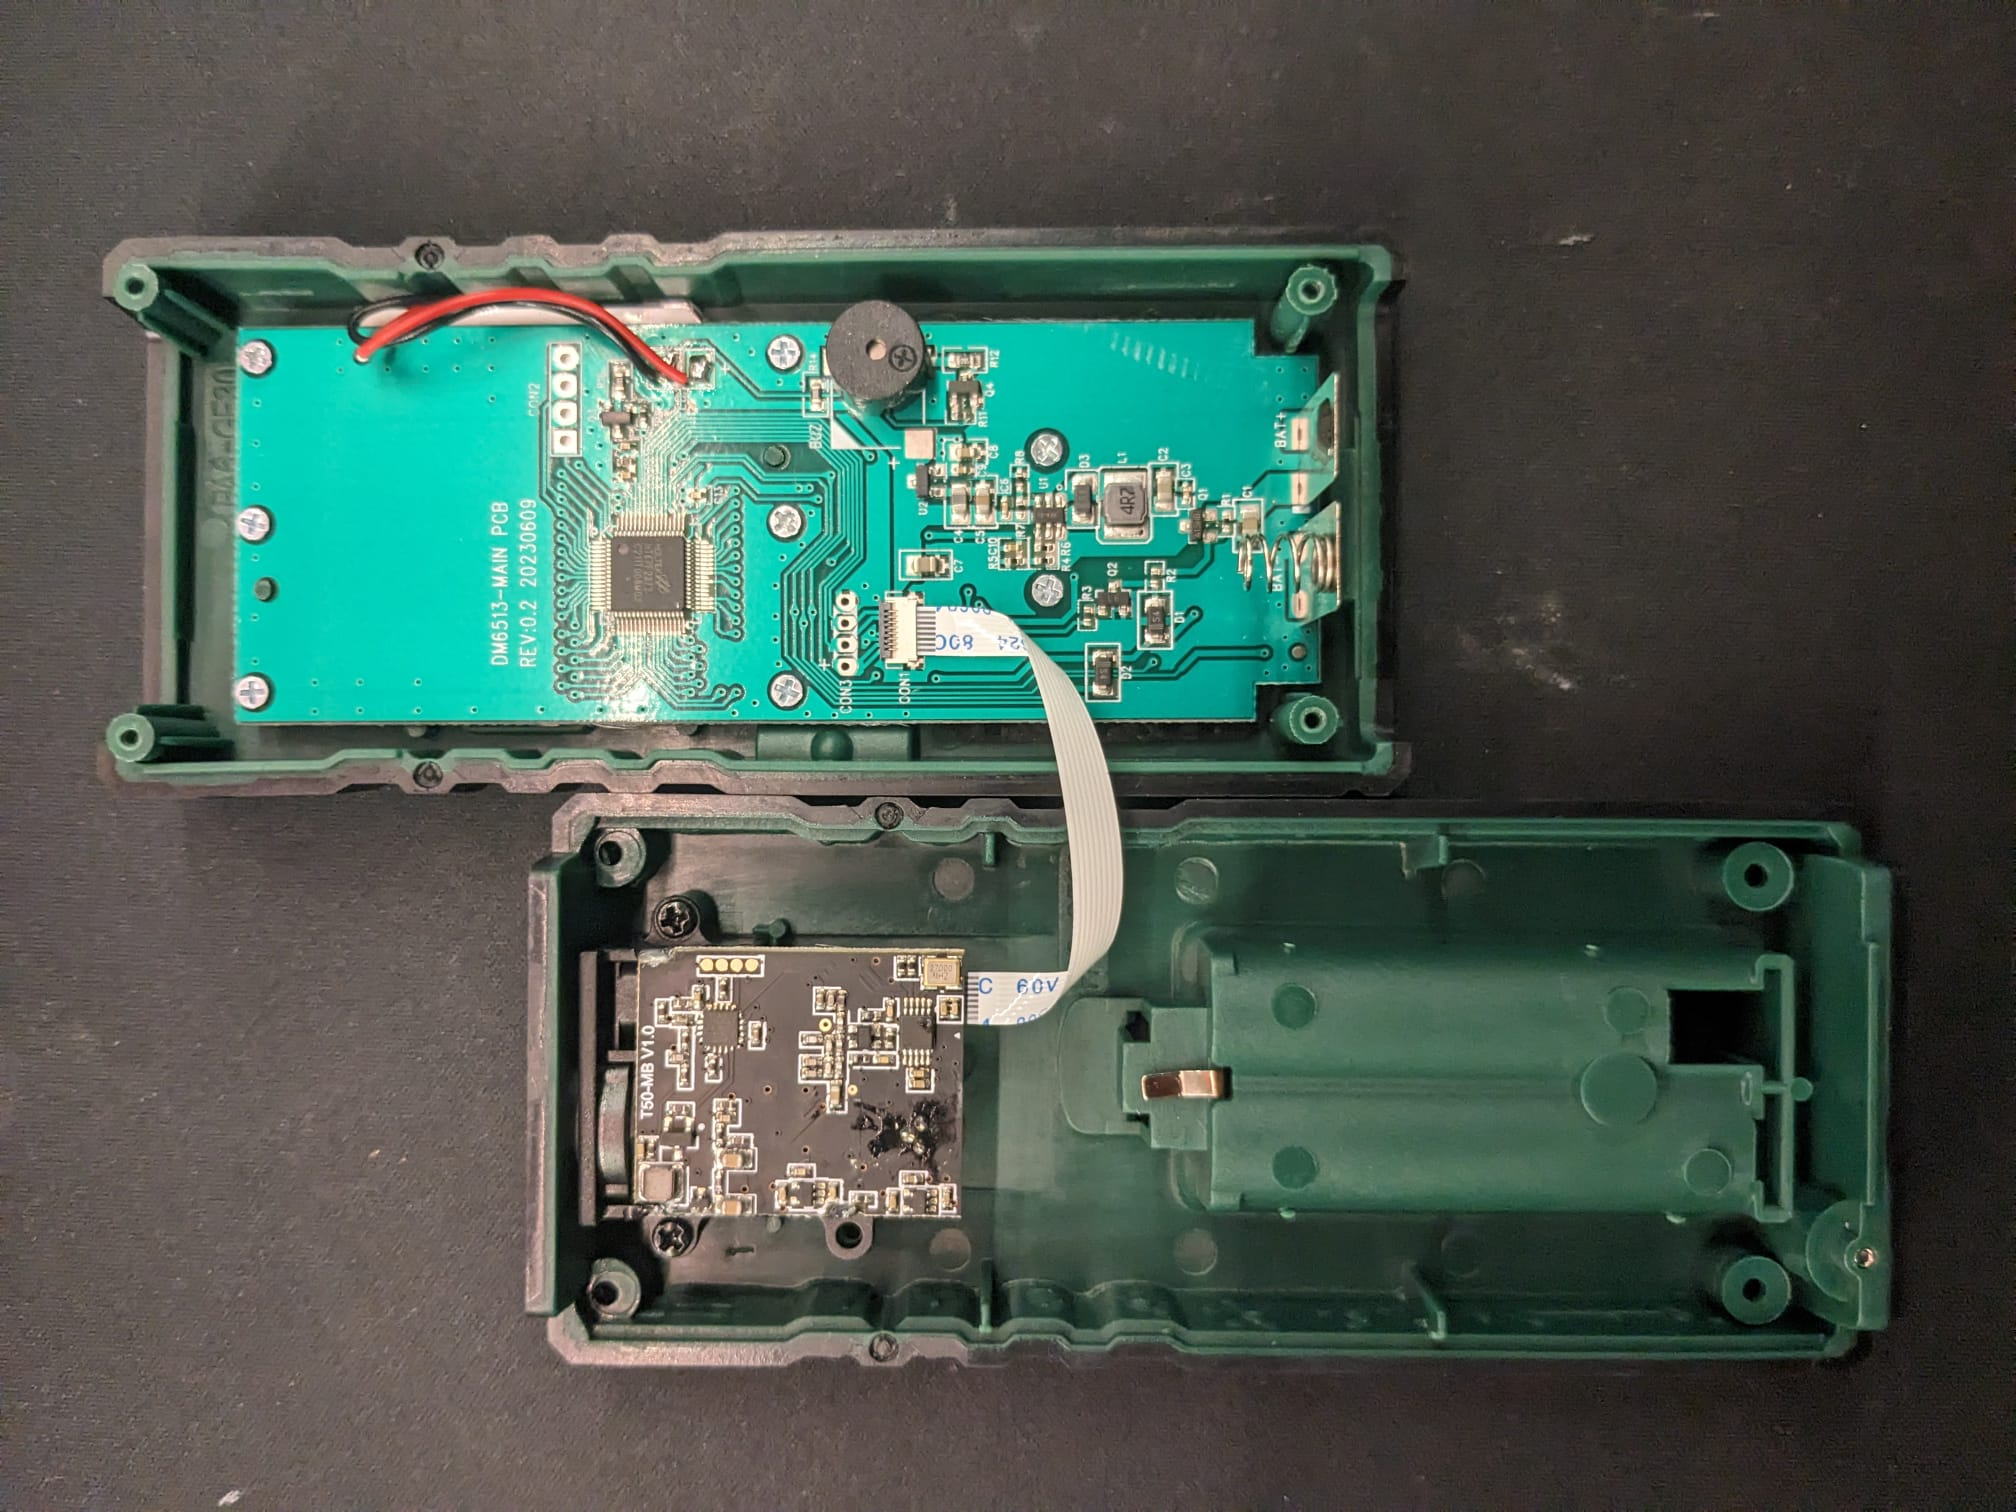
\includegraphics[width=1\textwidth]{img/2_sen/dis_parkside_1_outside.png}
		\caption{PARKSIDE – Distanzsensor – Innenaufbau}
		\label{img_2_2:sen_dis_parkside:1}
	\end{center}
\end{figure}


\begin{table}[ht]
	\centering
	\caption{PARKSIDE – Pin Mapping – Distanzsensor}
	\label{parkside:pinmapping}
	\begin{tabular}{l|ll}
		\hline
		\textbf{Pin} & \textbf{Farbe} & \textbf{Funktion} \\ \hline
		1            & Rot            & 3V3               \\
		2            & Weiß           & RX (receiver)     \\
		3            & Gelb           & TX (transmitter)  \\
		4            & Schwarz        & GND               \\ \hline
	\end{tabular}
\end{table}




\begin{itemize}
	\item + Anschlüsse herauszufinden vier anschlüsse gefunden.
	\item + Was für Aufgaben haben die Anschlüsse?
	      \subitem Was für ein Kommunikationsprotokol hat der Sensor?
	      \subitem Asynchron und seriell mit Baudrate 115200. (Ozilloskop)
	\item mit einem ESP32 die Sensordaten lesen.
	\item Nachrichtdekodierung (Controller MCU)
	      \subitem Ox24 Start (Nachricht start)
	      \subitem 0x26 Stopp (Nachricht ende)
	      \subitem 24 30 30 30 33 32 36 30 30 32 39 26 (Stopp signal)
	      \subitem 24 30 30 30 33 32 36 30 31 33 30 26 (Laser an)
	      \subitem 24 30 30 30 32 32 31 32 33 26 (Messen)
\end{itemize}

\section{Steuerung}


\chapter{Konklusion}

\chapter{Anhang}
\section{Schaltplan}
\label{Anhang:Schaltplan}

\myboxy{
	\begin{itemize}
		\item BMK beschriftung anpassen
		\item Bauteile einpflegen
	\end{itemize}
}{To-do}{\textwidth}
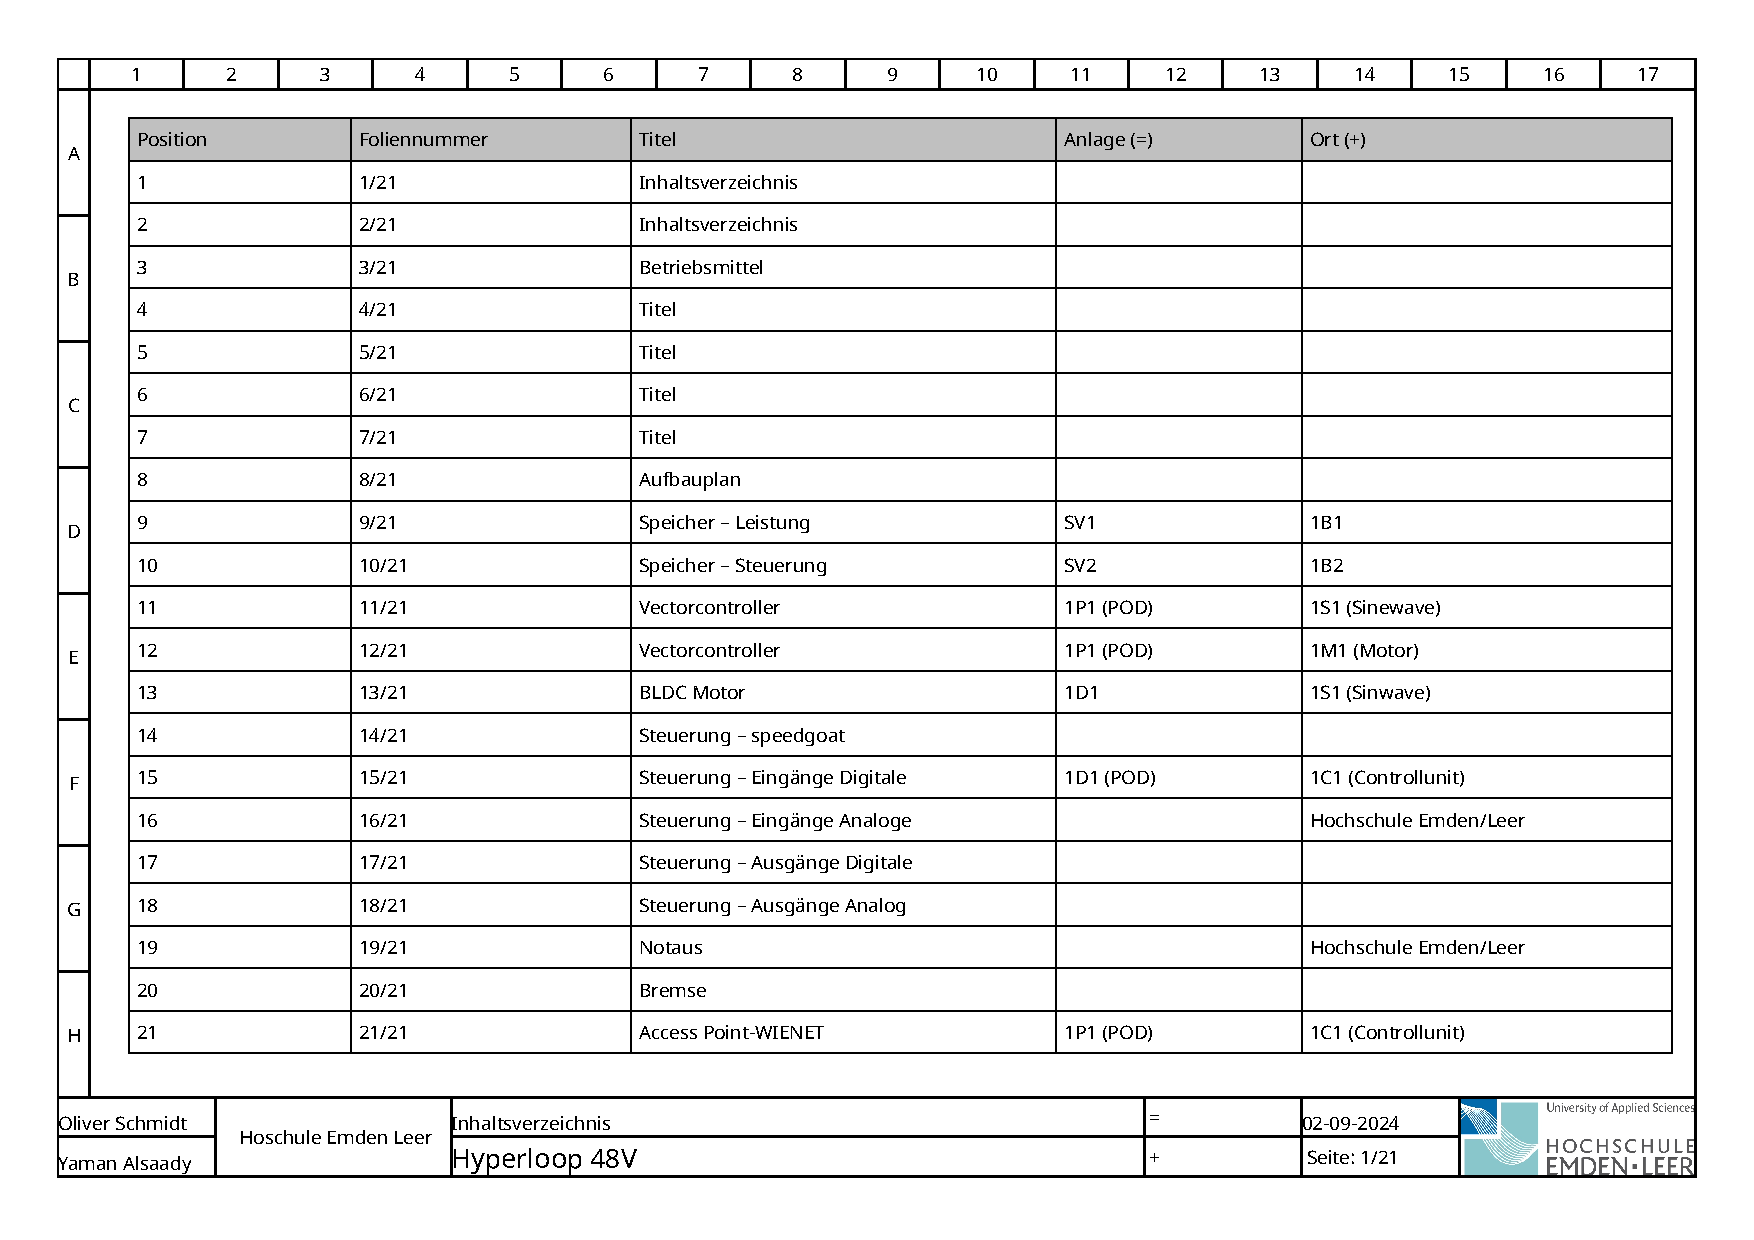
\includepdf[pages=-,landscape] {Anhang/Schaltplan.pdf}

\appendix
\include{source/Literaturverzeichnis}

\printbibliography

\end{document}
